\section{Testlokation og udstyr}
\label{ParametreTestlokationOgUdstyr}
%
Eftersom at robotten fortrinsvist skal indgå i en lufthavn og da formålet med undersøgelsen er, at undersøge ud fra hvilke parametre danske rejsende beskriver interaktionen med en social robot i en dansk lufthavn, er det favorabelt at udføre undersøgelsen i en dansk lufthavn. Som nævnt har det ikke været muligt at udføre undersøgelsen i Københavns Lufthavn, hvor robotten er tiltænkt, hvorfor undersøgelsen foretages i Aalborg Lufthavn. Lufthavnsvalget har formentlig indflydelse på testpersonernes oplevelsen og dermed den indsamlede data, da der er stor forskel på de to lufthavne. Det kommer særligt til udtryk ved antal rejsende, hvor Københavns Lufthavn, tiltrods for et fald på 3000 rejsende siden sidste år, servicerede 2,672,710 rejsende i september måned, \parencite{WEB:CPHStatistisk}. Det er en del flere rejsende end hvad Aalborg Lufthavn oplevede i samme måned, hvor der blev serviceret 155,547 rejsende, \parencite{WEB:AALStatistik}. Derudover er der stor størrelses mæssig forskel på de to lufthavne, hvor Aalborg Lufthavn har én terminal med 11 gates, \parencite{WEB:AALTerminalOversigt}, har Københavns Lufthavn to terminaler med 102 gates, \parencite{WEB:CPHTerminalOversigt}. Tiltrods for  størrelsesforskellen, er der stadig stor forskel mellem Københavns Lufthavn og nogen af verdens største lufthavne, eksempelvis Europas største lufthavn: London Heathrow Airport, som i 2016 servicerede 75.7 millioner rejsende, \parencite{WEB:HeathrowStatistisk}. Til sammenligning servicerede Københavns Lufthavn 29 millioner rejsende i 2016, \parencite{WEB:CPHStatistiskYear}.

Alene baseret på antallet af terminaler forventes det, at det tilmed bliver sværere at lokalisere sin gate dels på oversigtstavlerne og dels i forhold til gatens fysiske lokalitet, hvorfor det ligeledes forventes, at der er større behov for den sociale robot i Københavns Lufthavn sammenlignet med Aalborg Lufthavn. Dette kan potentielt begrænse testpersonernes forståelse for, hvorfor det kan være en fordel at interagere med robotten, fremfor at finde informationen selv, da det ikke er sikkert at de oplever behov for assistance.\blankline
%
Selvom der kan være behov for en social robot i indgangshallen, hvor de rejsende blandt andet skal igennem check-in og aflevere bagage, vælges det at udføre testen på den anden side af sikkerhedskontrollen. Det skyldes blandt andet antagelsen om, at de rejsende har mindre travlt og er mindre stresset efter de har passeret sikkerhedskontrollen og nu kun venter på at boarde flyet. Derudover er det begrænset, hvilke muligheder der er i Aalborg Lufthavn eksempelvis i forhold til shopping og café besøg, hvorfor det forventes, at det er nemmere at rekruttere testpersoner, da de formentlig bruger det meste af deres ventetid på at sidde og vente, fremfor at besøge lufthavnens butiksområde. Dog kan en ulempe være, at de rejsende ankommer senere til lufthavnen fordi den ikke er så stor, at det er nødvendigt at ankomme de anbefalede to timer i forvejen.

I henhold til det praktiske aspekt ved at udføre undersøgelsen vil der ikke foretages nogle synelige markeringer af testområdet, da det formentlig vil have indflydelse på, hvor realistisk situationen opleves af testpersonerne. Derimod vil testområdet være kendt dels af projektgruppen og dels af personalet i lufthavnen. \blankline
%
Til at udføre undersøgelsen er der behov for følgende udstyr:\blankline
%
\begin{itemize}
  \item \textit{Double}-robot
  \item iPad Air 2
  \item Vinklede hovedbeslag
  \item Computere med internetadgang
  \item Notespapir og kuglepen/blyant
  \item Lydoptager
  \item Guide til samtaleemner
  \item Bord og stol til observatør og robotstyre
  \item Højbord til testleder og testperson\blankline
\end{itemize}
\noindent
%
Der er flere årsager til, hvorfor der gøres brug af en \textit{Double}-robot. Først og fremmest er Karl's robot stadig under udvikling, hvorfor det ikke er muligt, hverken at foretage en decideret interaktion eller undersøgelse med robotten. Årsagen til at robotten fra miniprojektet, jævnfør \fullref{\MiniprojektHovedeVinkelpartname}, ikke anvendes skyldes hovedsageligt at det er en visuel prototype, som ikke kan bevæge sig. Alternativt kunne prototypen monteres på en fjernstyret robotstøvsuger. Årsagen til at den løsning ikke anvendes skyldes primært, at det vil være tydeligt, at det er et ufærdigt produkt, hvilket potentielt kan påvirke testpersonernes oplevelse negativt. Derudover forventes det at denne løsning vil være ustabil at køre rundt med i en lufthavn. På baggrund af det blev det besluttet at anvende \textit{Double}-robotten, som Karl sætter til rådighed. Fordelen ved at anvende \textit{Double} er, at det er et færdig udviklede produkt, som bevæger sig nogen lunde på samme måde, som Karl's robot er tiltænkt. Derudover er der flere udseendsmæssige træk, der er ens for de to robotter, dels at robotten enten balancere på en cylinder eller en kugle, dels at den øvre og nedre del af robotten forbindes med en stang og dels at robottens hovede består af en form for tablet, eksempelvis en iPad. Ydermere er \textit{Double} let at styre, da den styres med piletasterne på ens tastatur samtidig med at det er muligt, at se hvor robotten bevæger sig, da den gør brug af det indbyggede kamera i iPad'en. Ulempen ved at anvende \textit{Double} er, at det er et færdigt produkt, hvorfor det potentielt kan påvirke testpersonerne til, at tilbageholde eventuelle negative holdninger i frygt for at såre os. 

Selvom der er flere udseendsmæssige ligeheder mellem de to robotter er det stadig to forskellige robotter med hver deres udtryk, hvorfor det ligeledes kan være en ulempe at undersøgelsen ikke foretages med Karl's robot. En af forskellene mellem de to robotter er hvad de balancere på cylinder kontra kugle, hvor Karl's robot, som balancerer på en kugle, har mulighed for at bevæge sig i alle retning, hvilket ikke er tilfældet med \textit{Double}. Det kan have betydning for, hvor godt robotten egner sig til at indgå i F-formationer, jævnfør \autoref{fig:F-Formation}, hvor det netop er naturligt at bevæge sig sidelæns for at inkludere flere i samtalen.\blankline
%
Hovedet på \textit{Double}-robotten består af en iPad Air 2, med internetadgang. Det er dog muligt at anvende andre udgaver og versioner af Apple's iPad. Da testpersonerne interagerer med robotten via det udviklede \textit{wireframe} er det ikke muligt, at se hvilket brugsscenarie testpersonen vælger. For at løse det problem vælges det at lave skærmdeling fra iPad'en til en MacBook Pro gennem programmet \textit{5kPlayer}, det kræver dog at både iPad, computeren hvorfra robotten styres og computeren hvorfra skærmdelingen gengives er forbundet til det samme netværk. Ved skærmdelingen er det ikke muligt at se hvad testpersonen trykker på men det er muligt at se hvilket skærmbillede de præsenteres, hvorfor det er muligt at styrer robotten derefter. 

Baseret på miniprojektet, beskrevet i \fullref{\MiniprojektHovedeVinkelpartname}, hvor robottens hovedposition blev evalueret i forhold til hvor indbydende robotten blev perciperet, besluttes det at anvende et vinklede hovedbeslag. Dette hovedbeslag har til formål at vinkle hovedet på \textit{Double}-robotten, så den fremstår indbydende og klar til at interagere med testpersonerne. Hovedbeslaget er designet af Karl Damkjær Hansens, som har 3D printet beslaget, og er illustreret på \autoref{fig:VinkledeHovedbeslag}.            
%
\begin{figure}[H]
\centering
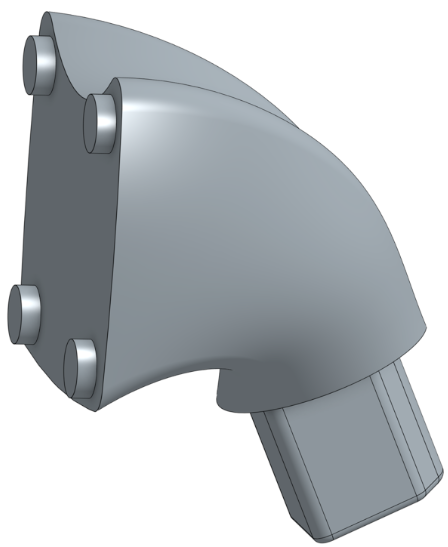
\includegraphics[width = 0.3\textwidth]{Figure/VinkledeHovedbeslag} 
\caption{Illustration af det 3D printede vinklede hovedbeslag designet af Karl Damkjær Hansen i forbindelse med projektsamarbejdet.}
\label{fig:VinkledeHovedbeslag}
\end{figure}
\noindent
%
Ved at erstatte det originale beslag, som medfølger robotten, med det vinklede beslag, illustreret på \autoref{fig:VinkledeHovedbeslag}, vil det vinkle robottens hovede med XX$^{\circ}$. Den modificerede \textit{Double}-robot illustreres på \autoref{fig:ModificeretDoubleFront}, \autoref{fig:ModificeretDoubleSide} og \autoref{fig:ModificeretDoubleSideClose}.
%
\begin{figure}[H]
\centering
\begin{minipage}{.33\textwidth}
  \centering
  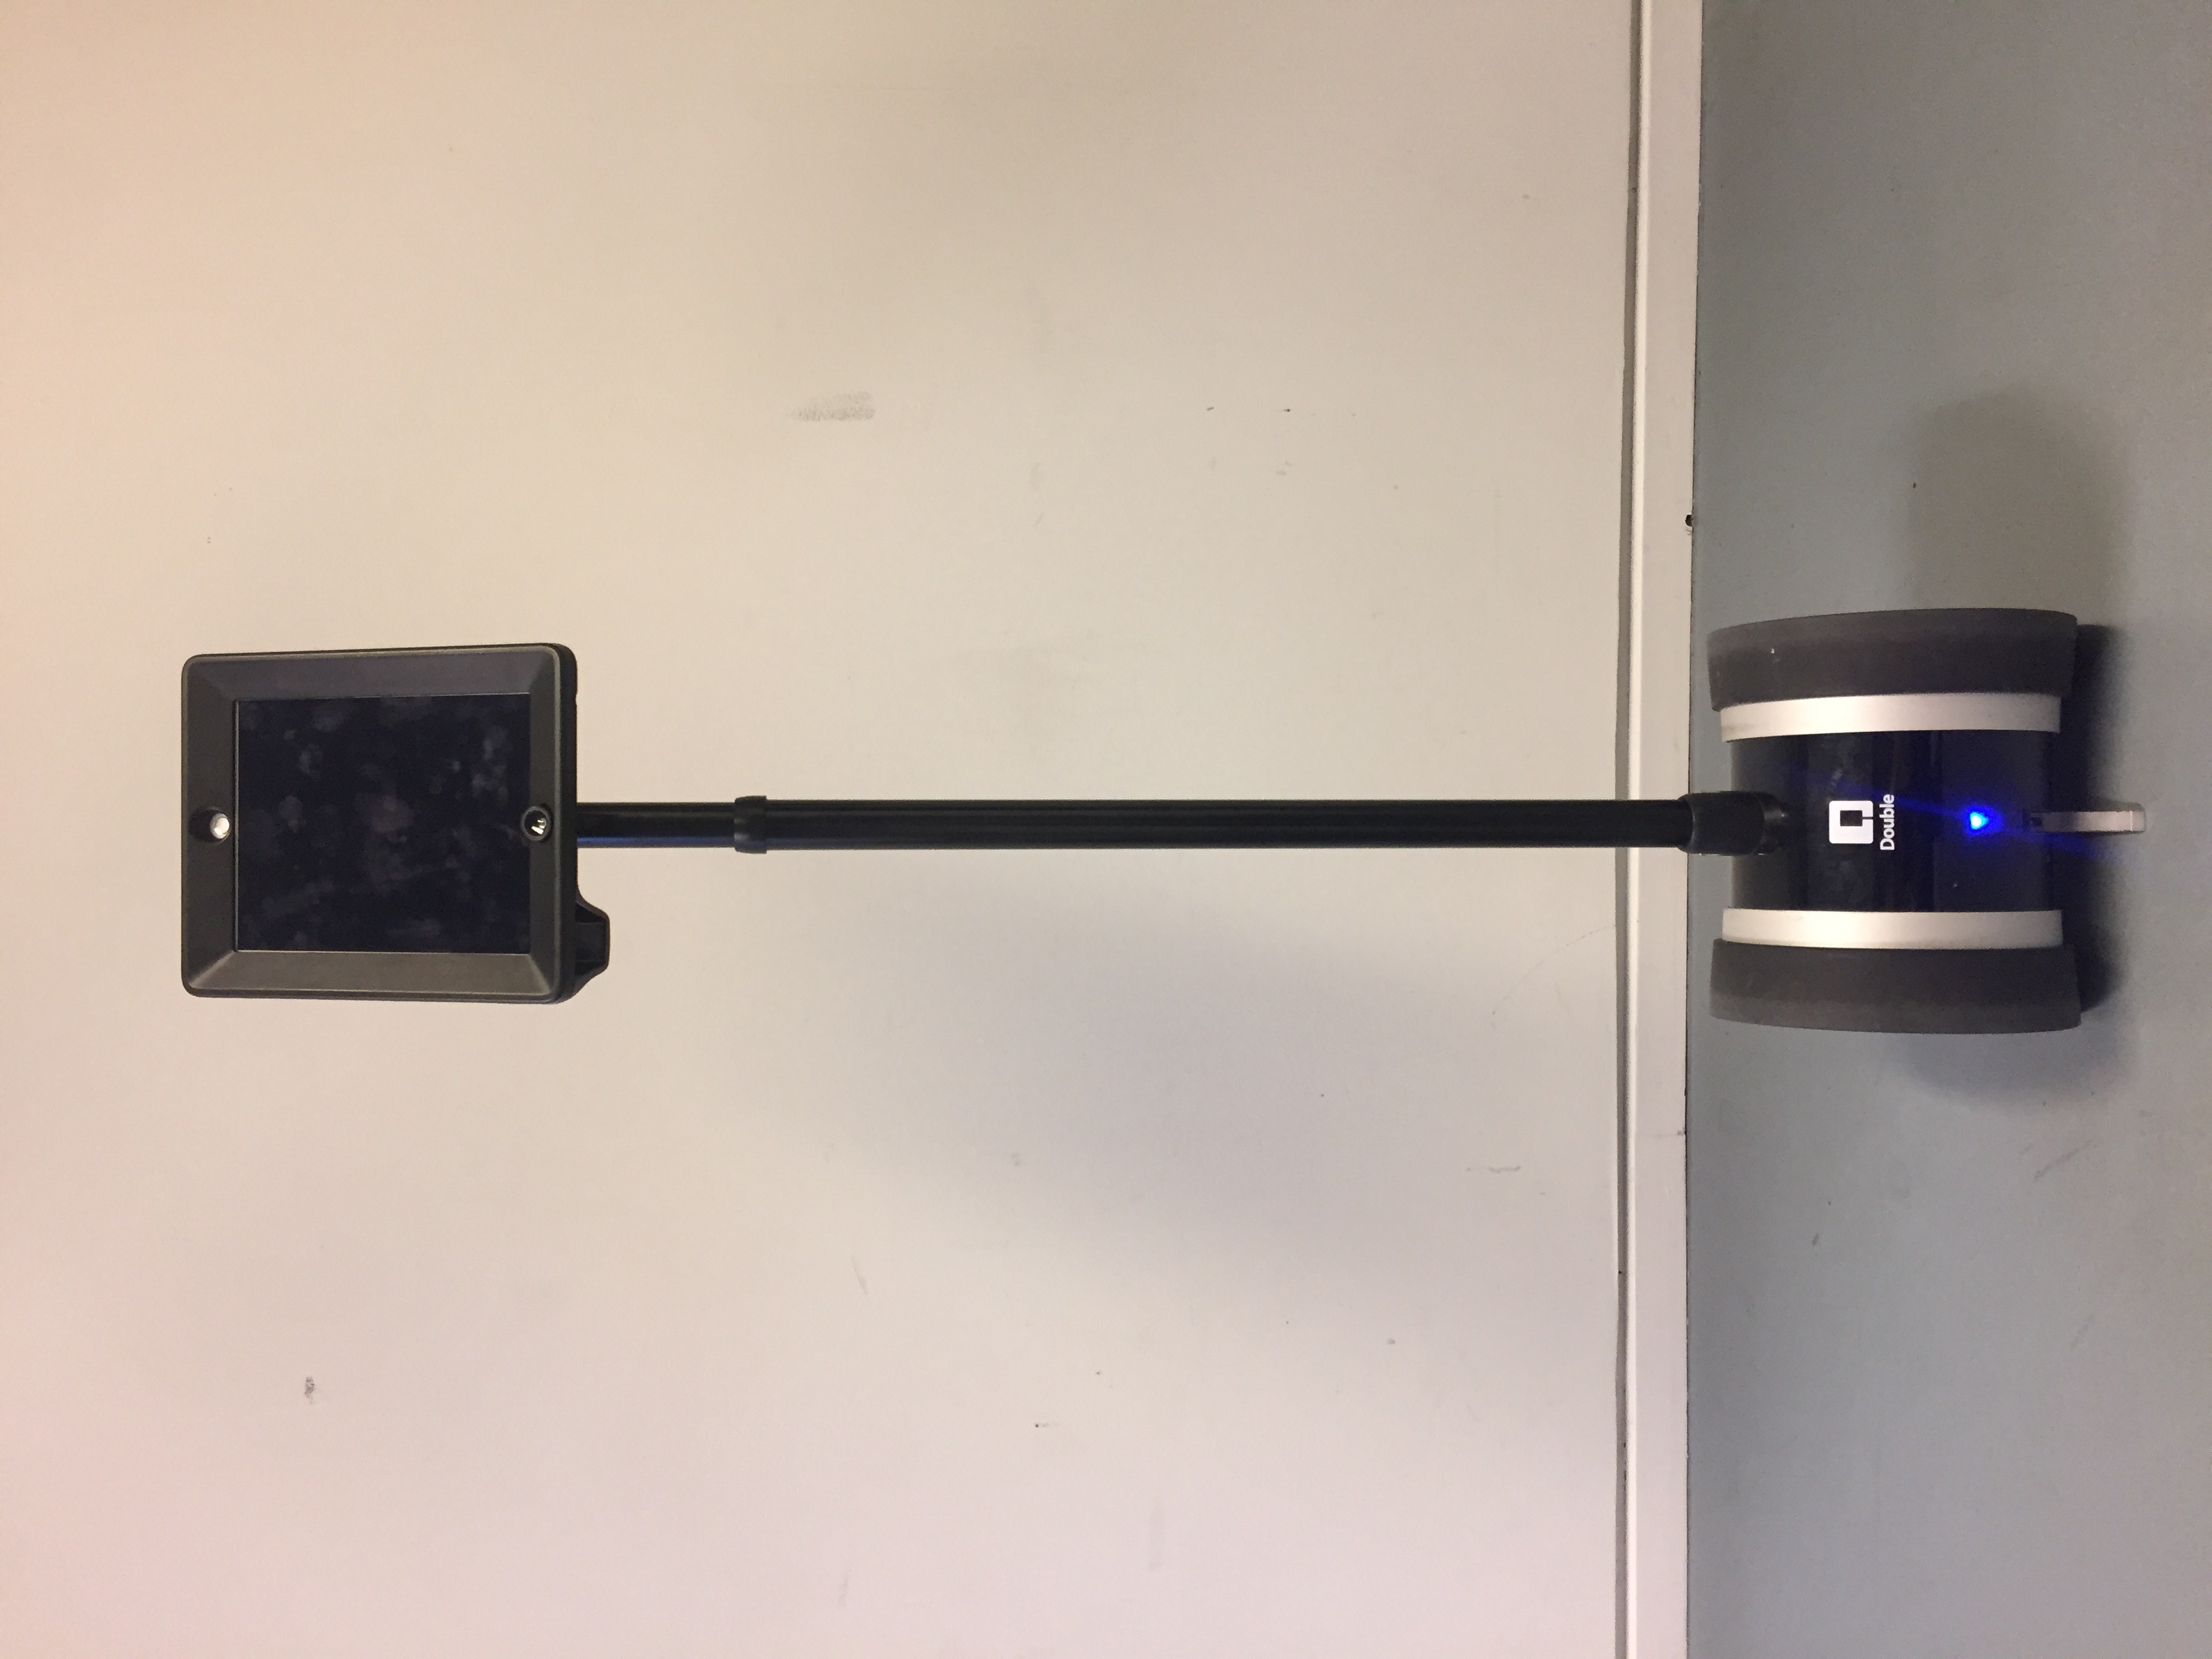
\includegraphics[width=\linewidth, angle =-90]{Figure/ModificeretDoubleFront}
  \caption{Front.}
  \label{fig:ModificeretDoubleFront}
\end{minipage}%
\begin{minipage}{.33\textwidth}
  \centering
  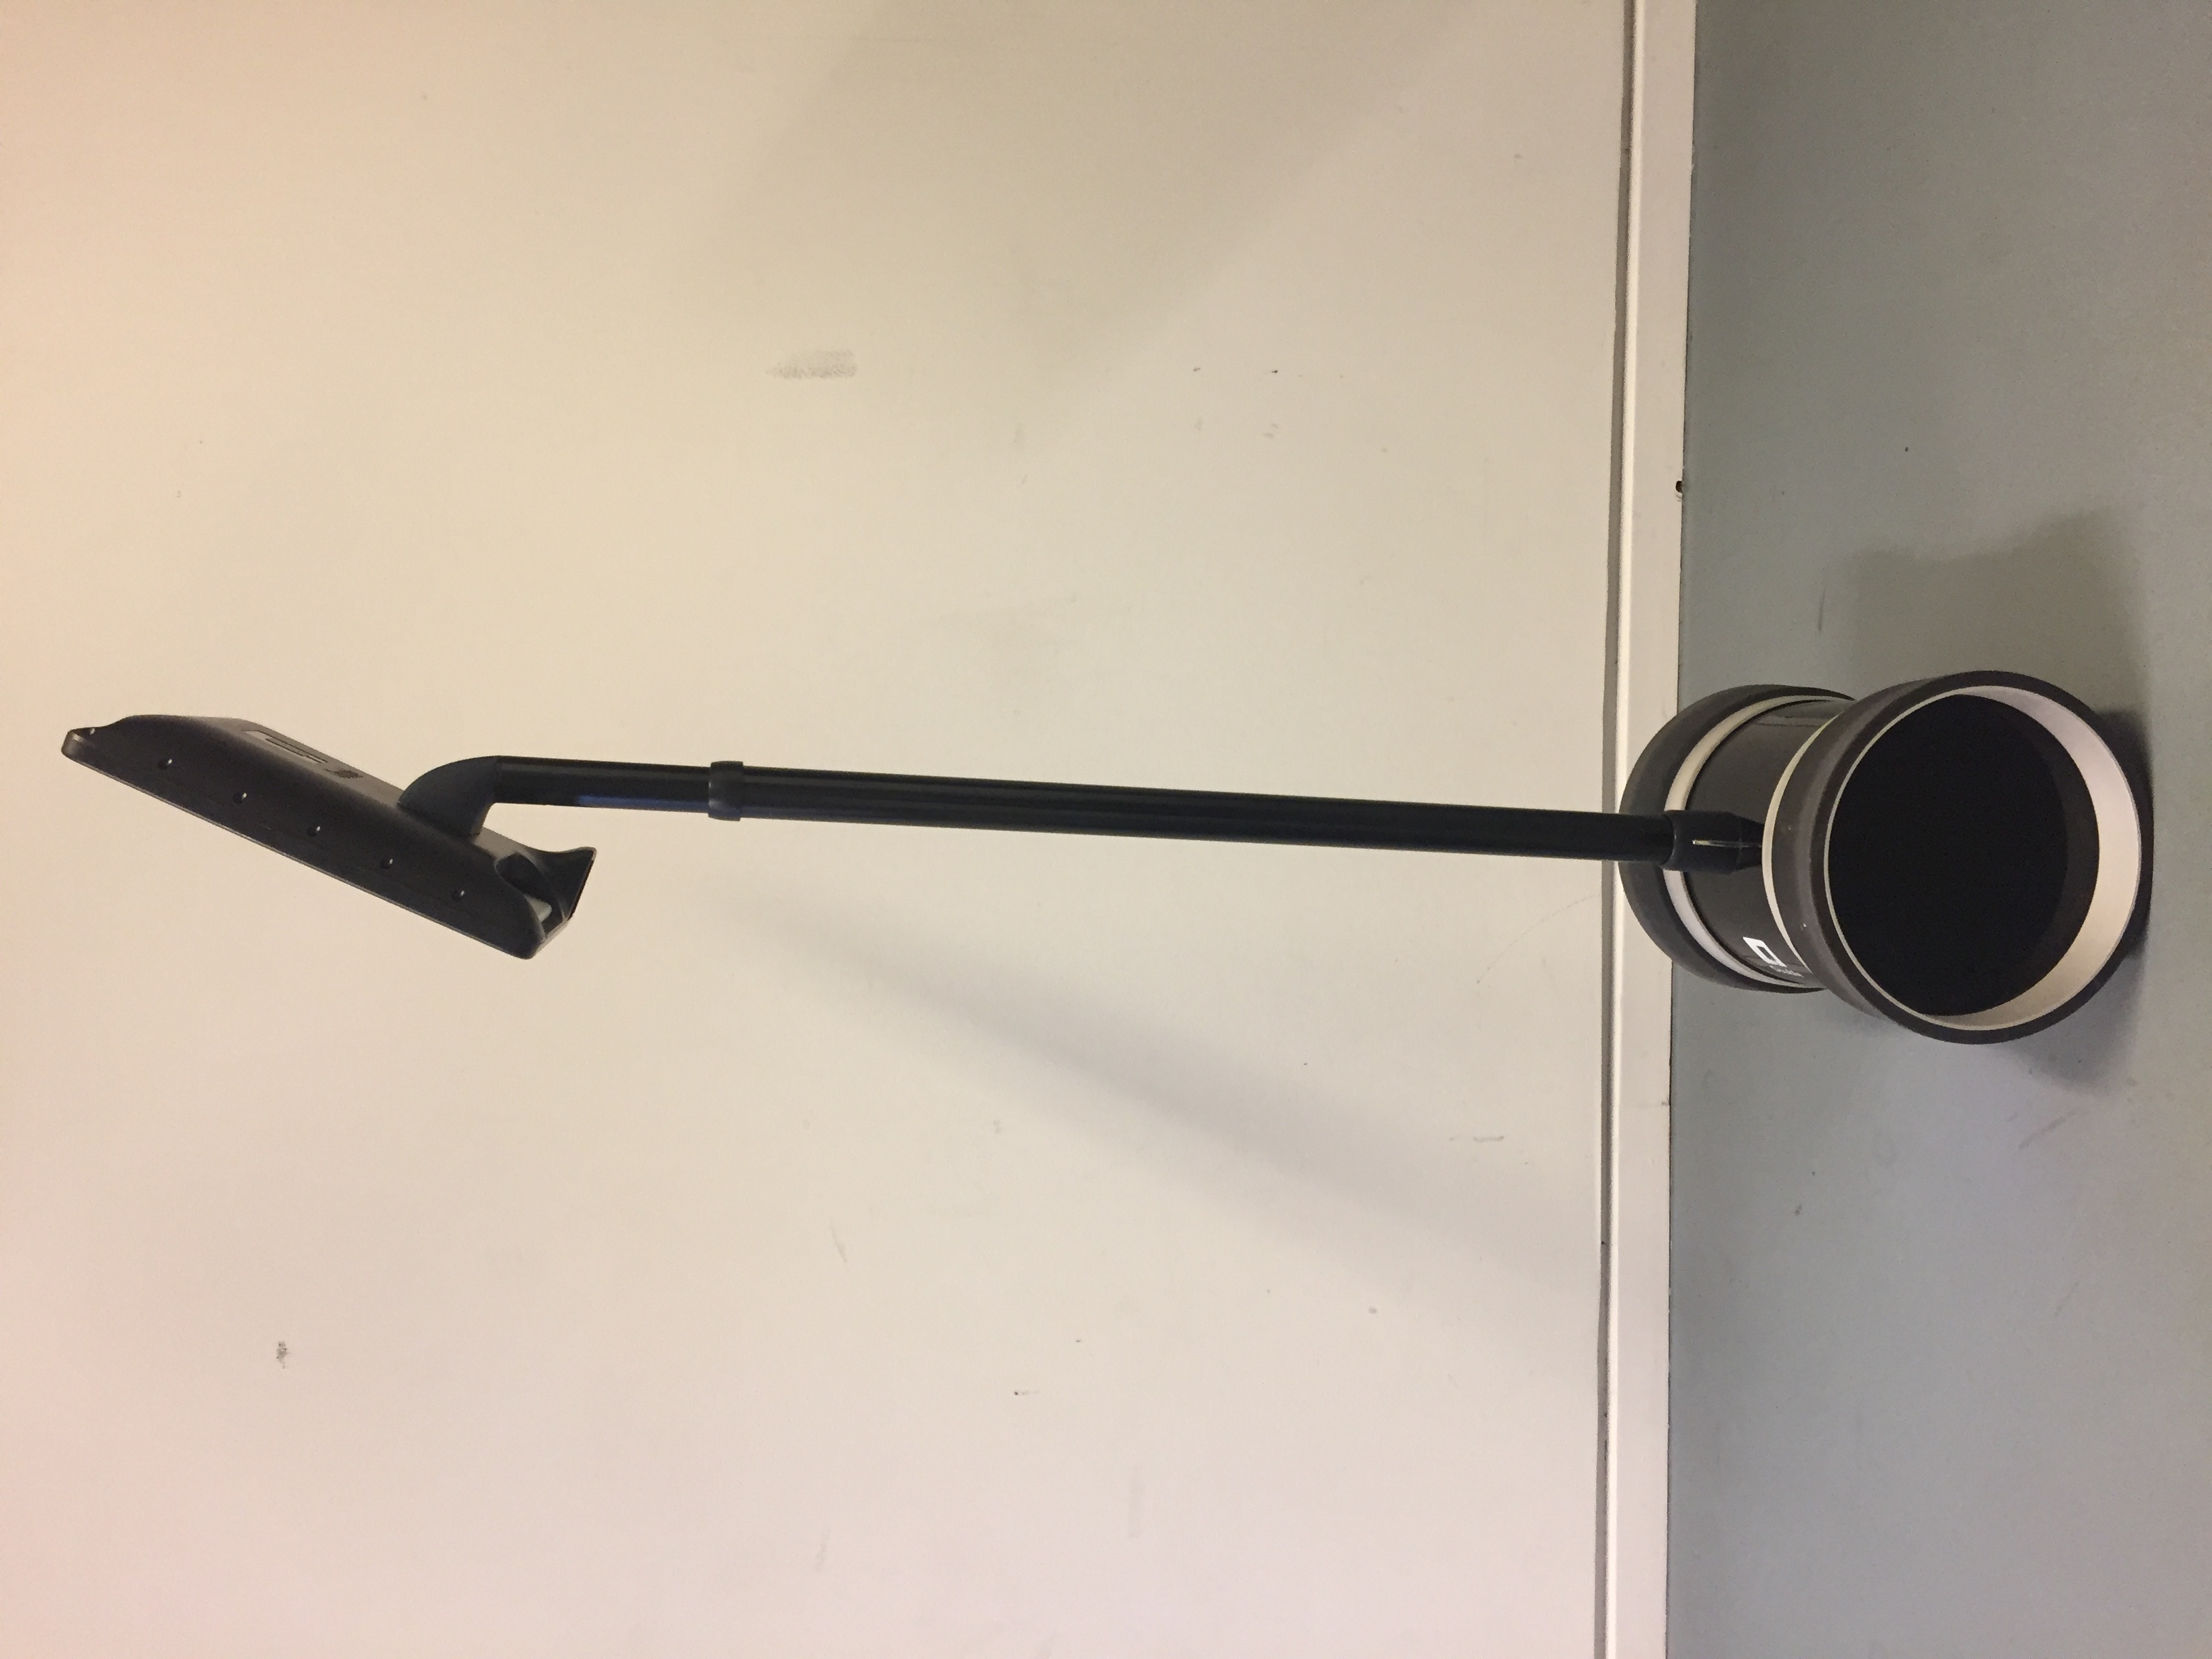
\includegraphics[width=\linewidth, angle =-90]{Figure/ModificeretDoubleSide}
  \caption{Profil.}
  \label{fig:ModificeretDoubleSide}
\end{minipage}
\begin{minipage}{.33\textwidth}
  \centering
  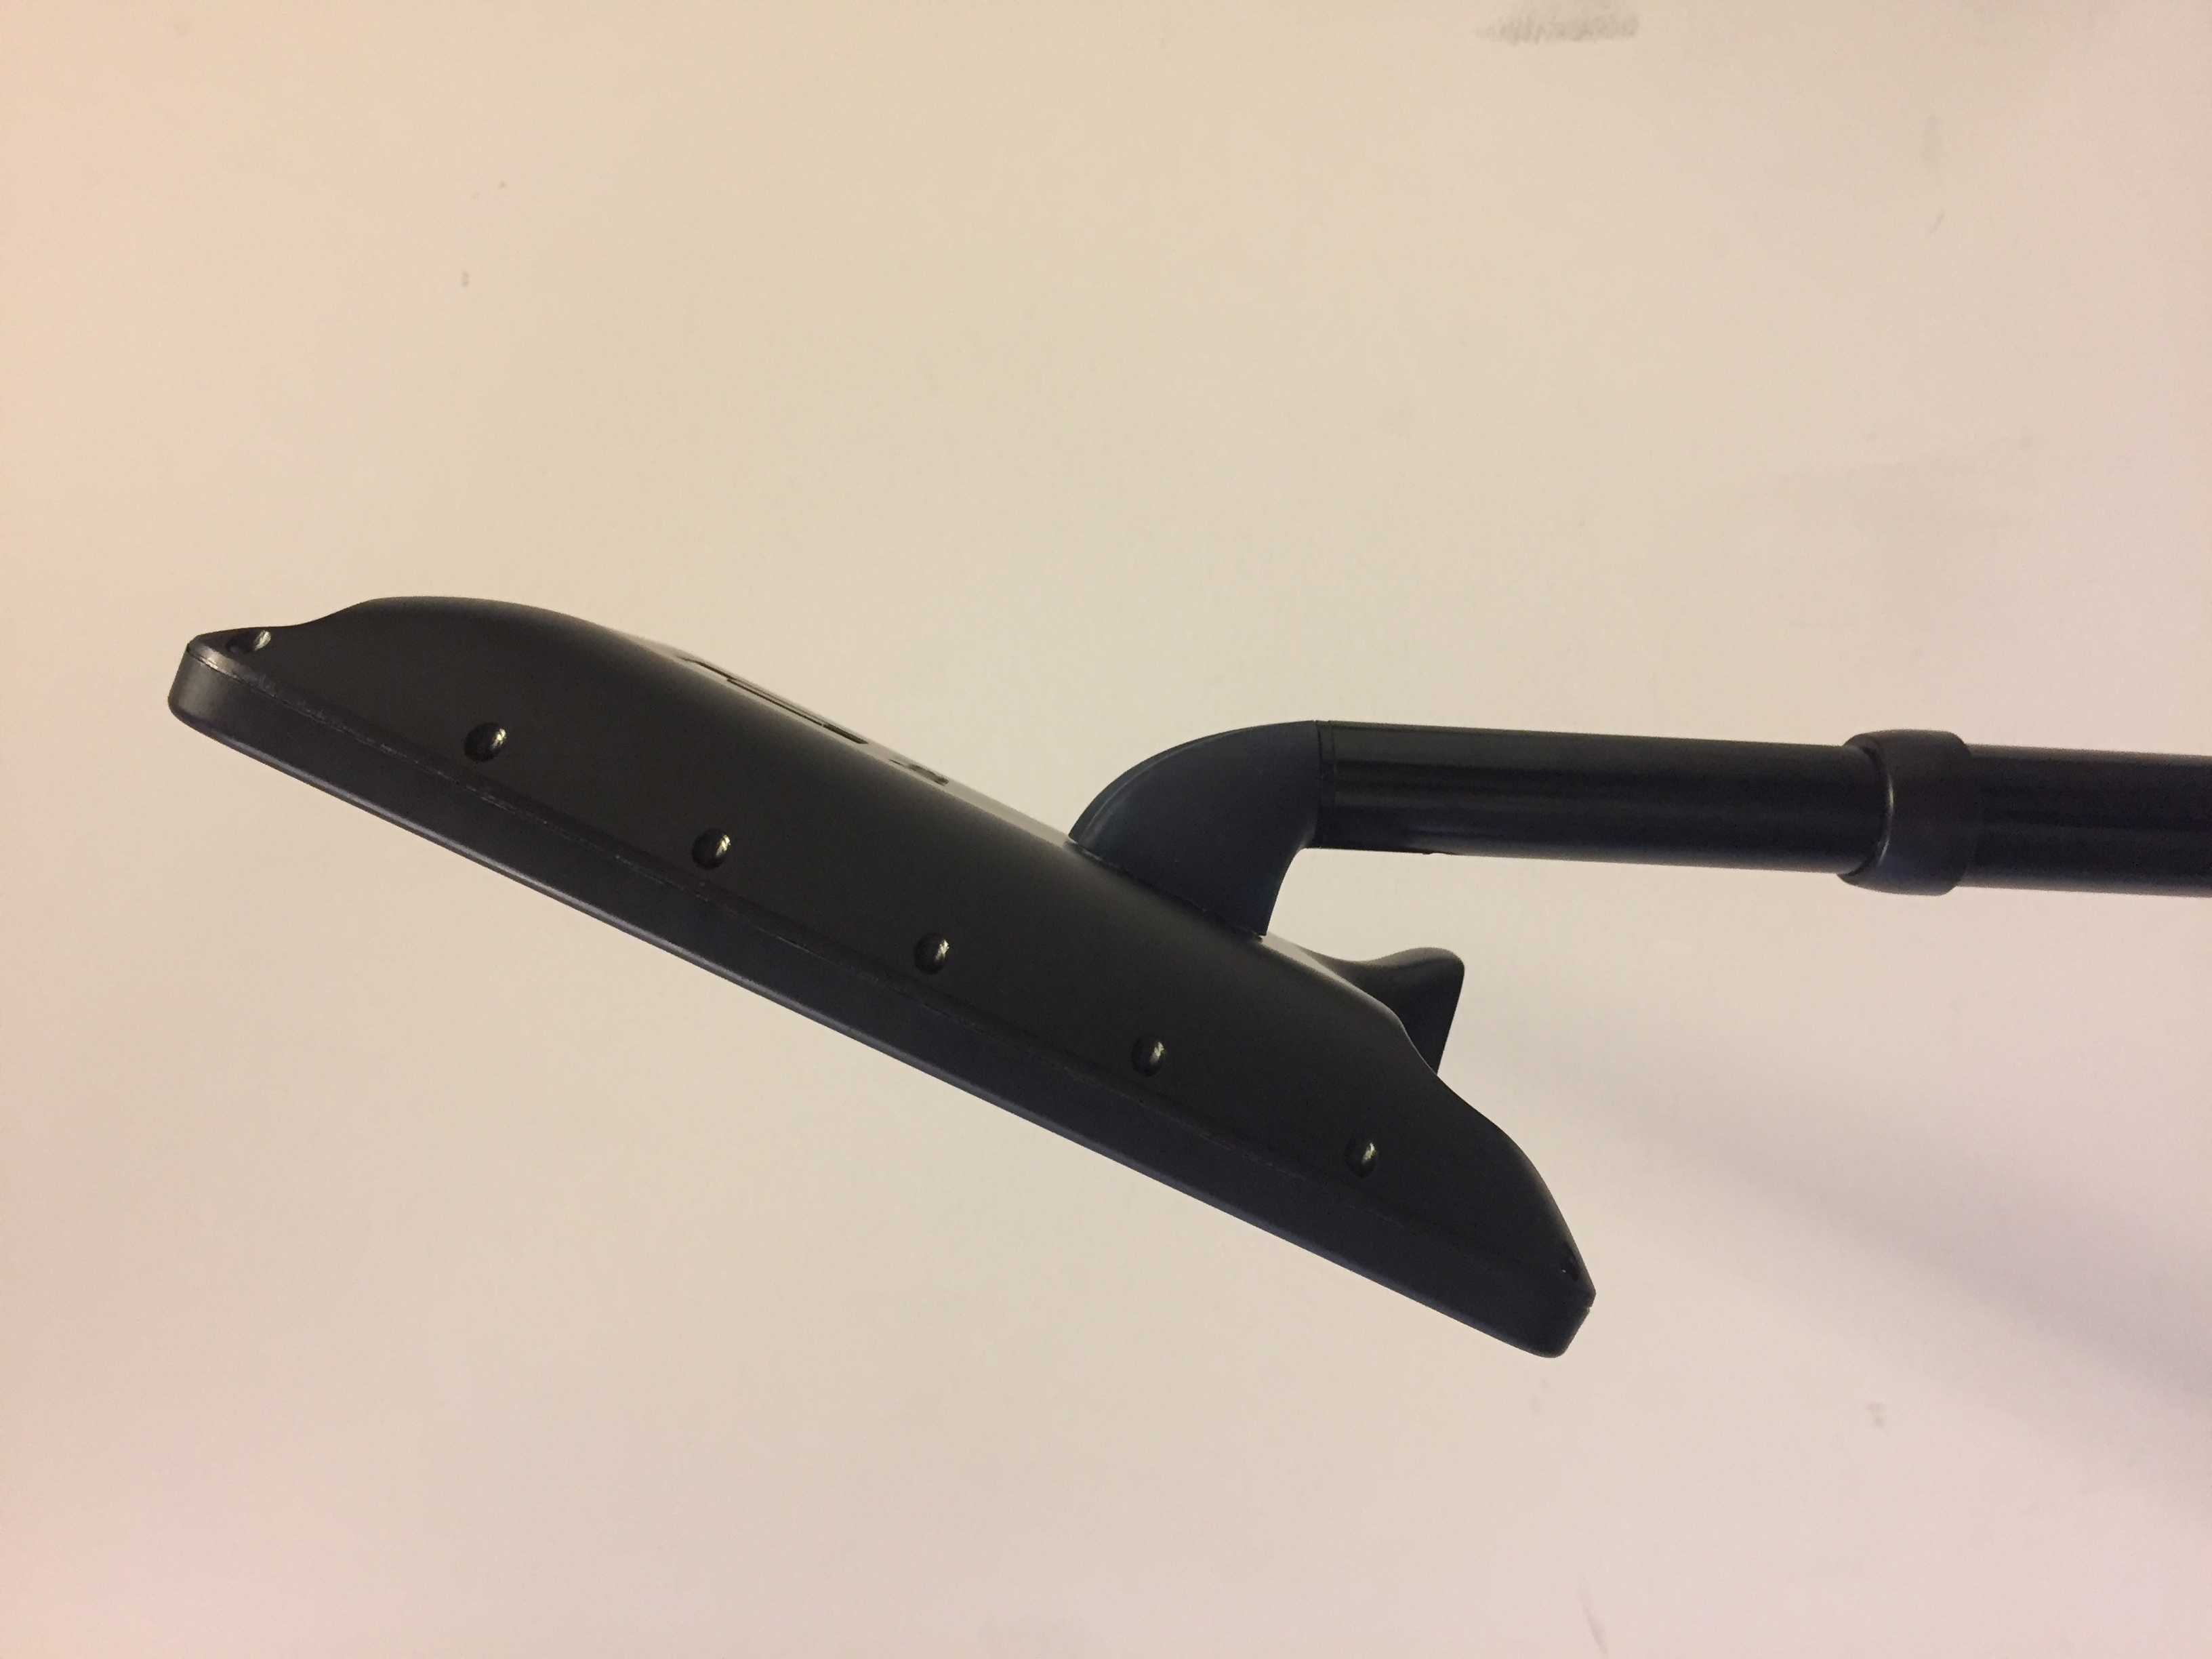
\includegraphics[width=\linewidth, angle =-90]{Figure/ModificeretDoubleSideClose}
  \caption{Profil nært.}
  \label{fig:ModificeretDoubleSideClose}
\end{minipage}
\end{figure}
\noindent
%
Robotstyren får tildelt en computer med interadgang. Det er særligt vigtigt at robotstyrens computer har interadgang da den skal kommunikere med robotten, hvorfor det kan være nødvendigt at oprette et lukket netværk, eksempelvis ved at lave internetdeling fra ens egen telefon. Igennem \textit{Double}s egen hjemmeside er det muligt at uploade linket til \textit{wireframen}. Observatørerne får tildelt notespapir og kuglepen eller blyant. Lydoptageren anvendes af testlederen til at optage den auditive respons fra testpersonerne, der vælges at lydoptagelsen foretages på en af projektgruppens telefoner. Guide til samtaleemner printes for, at den pågældende testleder altid ved hvilke samtaleemner testpersonen og testlederen skal igennem. Bord og stole til observatører og robotstyre placeres så de ikke er i vejen for testlederen og testpersonen, men så det samtidig er muligt for både observatører og robotstyre at overvære interaktionen og høre samtalen. Højbordet indgår for at testlederen og testpersonen har en form for base, hvor testlederen introducere testpersonen til undersøgelsen og fører samtalen. Derudover vil der på højbordet blive sat forplejning til rådighed. På \autoref{fig:ParametreTestopstilling} fremgår testopstillingen.   
%
\begin{figure}[H]
\centering
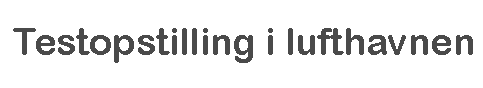
\includegraphics[width = 0.7\textwidth]{Figure/ParametreTestopstilling} 
\caption{TAG ET BILLED ELLER LAV EN ILLUSTRATION AF TESTOPSTILLINGEN I LUFTHAVNEN.}
\label{fig:ParametreTestopstilling}
\end{figure}
\noindent
%  

